\documentclass{beamer}
\usepackage[english,spanish]{babel}
\usetheme{Boadilla}

\usepackage{graphicx}
\usepackage{xcolor}

\usepackage{makecell}

\usepackage{csquotes}
\usepackage{hyperref}
\usepackage[style=ieee]{biblatex}
\addbibresource{referencias.bib}

\title[EDA de Valores Nutricionales por Dieta]{Análisis Estadístico de Valores Nutricionales por Tipo de Dieta}

\setbeamercolor{frametitle}{fg=black}
\setbeamercolor{footline}{fg=black, bg=black!25}
\setbeamertemplate{footline}{
    \begin{beamercolorbox}[wd=\paperwidth, ht=2mm, dp=2mm, center]{footline}
        \begin{columns}[T]
            \begin{column}{0.5\textwidth}
                \centering
                \insertshorttitle
            \end{column}
            \begin{column}{0.5\textwidth}
                \centering
                \insertsection
            \end{column}
        \end{columns}
    \end{beamercolorbox}
}
\setbeamertemplate{navigation symbols}{}

\usepackage{hyperref}
\hypersetup{
    colorlinks=true,
    urlcolor=blue,
    linkcolor=black,
    citecolor=blue
}

\begin{document}

    \begin{frame}[plain]
        \begin{columns}[T]
            \begin{column}{0.08\textwidth}
                \centering
                
\includegraphics[width=\textwidth]{Resources/logo_unam.jpg}
            \end{column}
            \begin{column}{0.60\textwidth}
                \centering
                {\small Universidad Nacional Autónoma de México\par
                Escuela Nacional de Estudios Superiores\par
                Morelia}
            \end{column}
            \begin{column}{0.08\textwidth}
                \centering
                
\includegraphics[width=\textwidth]{Resources/logo_enes.jpg}
            \end{column}
        \end{columns}
        \vspace{1.5cm}
        \begin{center}
            {\bfseries Reporte}\par
            {\Large Análisis Estadístico de Valores Nutricionales}\par
            {\Large por Tipo de Dieta}\par
            \vspace{0.5cm}
            {\bfseries Alexis Aguilar}
        \end{center}
        \vspace{1.5cm}
        \begin{columns}[T]
            \begin{column}{0.5\textwidth}
                \raggedright
                {\footnotesize Estadística Descriptiva e Inferencial}
            \end{column}
            \begin{column}{0.5\textwidth}
                \raggedleft
                {\footnotesize A: \underline{7 de Abril del 2025}}
            \end{column}
        \end{columns}
    \end{frame}

    \begin{frame}[plain]{Índice}
        \tableofcontents
    \end{frame}

    \section{Presentación de los Datos}

    \begin{frame}{Fuente de Datos}
        \begin{itemize}
            \item<1->El conjunto de datos consta de recetas 
            de diferentes dietas y cocinas, incluye también 
            la información de los macronutrientes (carbohidratos, 
            proteínas, lípidos) que aportan cada receta. Se 
            encuentra publicado en \cite{dataset_macronutrients}
            \item<2->El crear planes alimenticios saludables, ya 
            sea usando las recetas proporcionadas o creando unas 
            nuevas basadas en una dieta y cocina, y el estudiar 
            la relación entre dieta y salud
            \item<3->Las recetas fueron proporcionadas por 
            diferentes creadores de las mismas y demás 
            contribuidores al conjunto de datos
        \end{itemize}
    \end{frame}

    \begin{frame}{Interés del Estudio}
        \begin{itemize}
            \item<1->\cite{marvastipopular}Como en cada dieta se consumen diferentes 
            alimentos y productos con ciertas características 
            para ya sea respetar alguna creencia, fundamento o 
            cuota de macronutrientes
            \item<2->Por lo que el interés del trabajo 
            es el probar si existe una diferencia o distinción 
            entre las dietas en base a sus aportes de macronutrientes
        \end{itemize}
    \end{frame}

    \begin{frame}{Variables del Conjunto de Datos [I]}
        El conjunto de datos con el se trabajará consta de 
        las siguientes variables:
        \begin{itemize}
            \item<2->\textbf{Diet\_type}: [Nominal] Representa 
            el tipo de dieta (DASH, keto, mediterránea, paleo, vegana) 
            a la que pertenece una receta. Permite estratificar las recetas 
            y estudiarlas de una manera más granular
            \item<3->\emph{Recipe\_name}: [Nominal] Nombre de 
            la receta. No es una variable relevante para el trabajo
            \item<4->\textbf{Cuisine\_type}: [Nominal] Representa 
            a qué (estilo de) cocina o región (mexicana, americana, 
            italiana, entre otras) pertenece una receta
        \end{itemize}
    \end{frame}

    \begin{frame}{Variables del Conjunto de Datos [II]}
        Otras variables que serán eje para el trabajo son:
        \begin{itemize}
            \item<1->\textbf{Protein(g)}: [Continua] Representa la 
            cantidad de proteínas en gramos contenidas en una receta
            \item<2->\textbf{Carbs(g)}: [Continua] Representa la 
            cantidad de carbohidratos en gramos contenidas en una receta
            \item<3->\textbf{Fat(g)}: [Continua] Representa la 
            cantidad de grasas en gramos contenidas en una receta
        \end{itemize}
    \end{frame}

    \section{Estadística Descriptiva}

    \begin{frame}{Ejemplo de Registros en el Conjunto de Datos}
        \begin{center}
        \begin{tabular}{|c|c|c|}
            \hline
            \textbf{Diet\_type} & Recipe\_name & \textbf{Cuisine\_type} \\
            \hline
            \small{dash} & \small{Spicy Haddock Fish Cakes} & \small{mediterranean} \\
            \small{keto} & \small{Keto Cauliflower, Eggs, and Bacon Salad} & \small{american} \\
            \small{mediterranean} & \small{Mediterranean Quinoa Salad} & \small{mediterranean} \\
            \small{paleo} & \small{Paleo Zuppa Toscana} & \small{italian} \\
            \small{vegan} & \small{Vegan Jelly-Filled Muffins Recipe} & \small{american} \\
            \hline
        \end{tabular}\\
        \vspace{0.5cm}
        \begin{tabular}{|c|c|c|}
            \hline
            \textbf{Protein(g)} & \textbf{Carbs(g)} & \textbf{Fat(g)} \\
            \hline
            \small{102.58} & \small{164.23} & \small{3.68} \\
            \small{56.73} & \small{63.32} & \small{143.25} \\
            \small{30.65} & \small{62.27} & \small{59.26} \\
            \small{179.75} & \small{261.94} & \small{425.47} \\
            \small{20.55} & \small{440.45} & \small{79.32} \\
            \hline
        \end{tabular}
        \begin{tabular}{|c|c|c|}
            \hline
            \textbf{Protein(g)} & \textbf{Carbs(g)} & \textbf{Fat(g)} \\
            \hline
            \small{0.60} & \small{0.37} & \small{0.01} \\
            \small{0.24} & \small{0.21} & \small{0.54} \\
            \small{0.40} & \small{0.20} & \small{0.38} \\
            \small{0.30} & \small{0.20} & \small{0.49} \\
            \small{0.81} & \small{0.03} & \small{0.14} \\
            \hline
        \end{tabular}
        \end{center}
    \end{frame}
    
    \begin{frame}{Estadísticos Poblacionales [I]}
        \begin{center}
            \begin{tabular}{|c|ccc|}
                \hline
                Medida Poblacional & Carbs(g) & Protein(g) & Fat(g) \\
                \hline
                Media               & 0.433471 & 0.234762 & 0.331767 \\
                $Q_1$               & 0.205251 & 0.110188 & 0.184583 \\
                $Q_2$               & 0.432028 & 0.190931 & 0.314359 \\
                $Q_3$               & 0.635058 & 0.338059 & 0.464532 \\
                Desviación Estándar & 0.256032 & 0.163886 & 0.194920 \\
                Mínimo              & 0.000330 & 0.000000 & 0.000000 \\
                Máximo              & 1.000000 & 0.887557 & 0.997940 \\
                Asimetría de Fisher & 0.189556 & 0.922401 & 0.461455 \\
                \hline
            \end{tabular}
        \end{center}
    \end{frame}

    \begin{frame}{Estadísticos Poblacionales [II]}
        \begin{itemize}
            \item<1->Debido a que son medidas sobre todos 
            los datos, sin estratificar, se tiene que no 
            hay una referencia de lo que se espera obtener
            \item<2->Se reportan bajos valores en proteínas 
            en comparación con los carbohidratos y grasas 
            si se hace uso de la mediana ($Q_2$)
            \item<3->Si se consider el rango intercuartil y 
            la desviación estándar, los valores de proteínas y 
            grasas se encuentran concentradas en ciertas regiones 
            en contraste con los posibles valores de los carbohidratos 
            que son más diversos
        \end{itemize}
    \end{frame}

    \begin{frame}{Estadísticos Poblacionales [III]}
        \begin{center}
            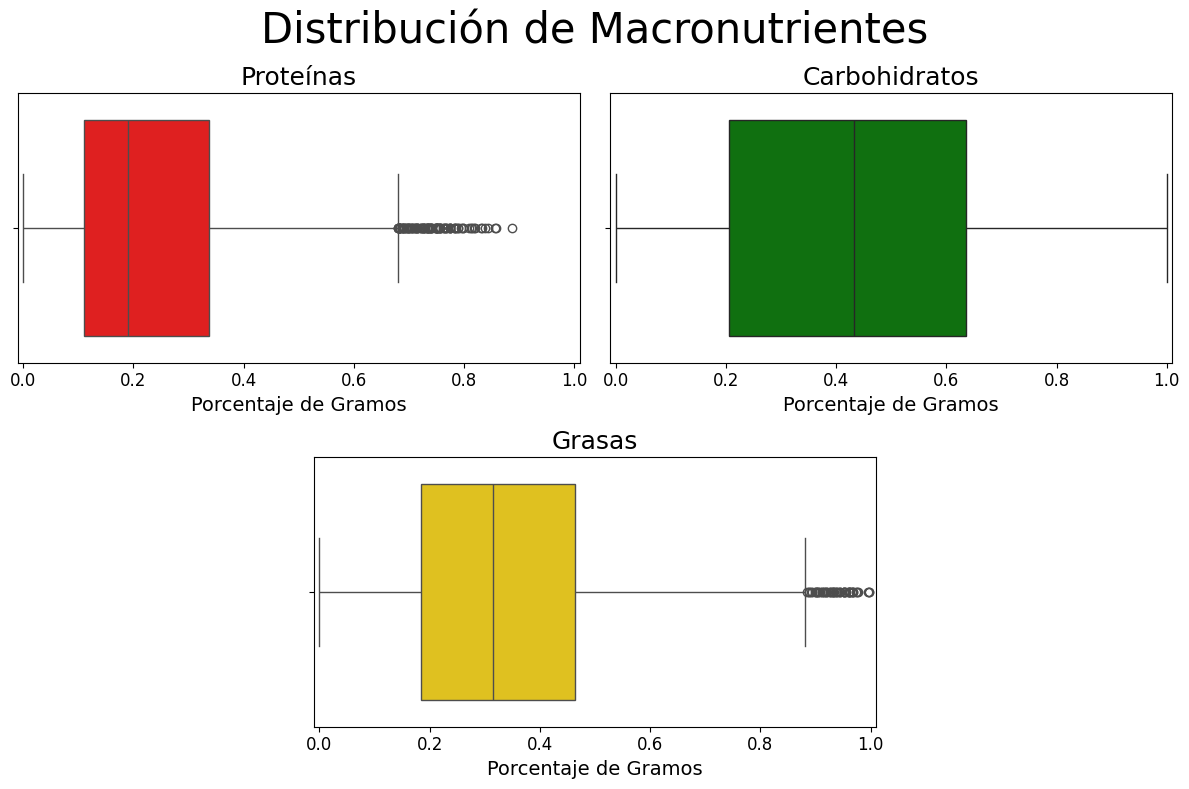
\includegraphics[width=0.9\textwidth]{Resources/2_02_plot_01.png}
        \end{center}
    \end{frame}

    \begin{frame}{Estadísticos Estratificados [DASH]}
        El $55\%$ de sus macronutrientes son carbohidratos 
        (provenientes de frutas, vegetales y granos enteros); 
        el $25\%$ son grasas que, por su naturaleza, son saludables; 
        y el $20\%$ son proteínas, las cuáles provienen de carnes margas
        \begin{center}
            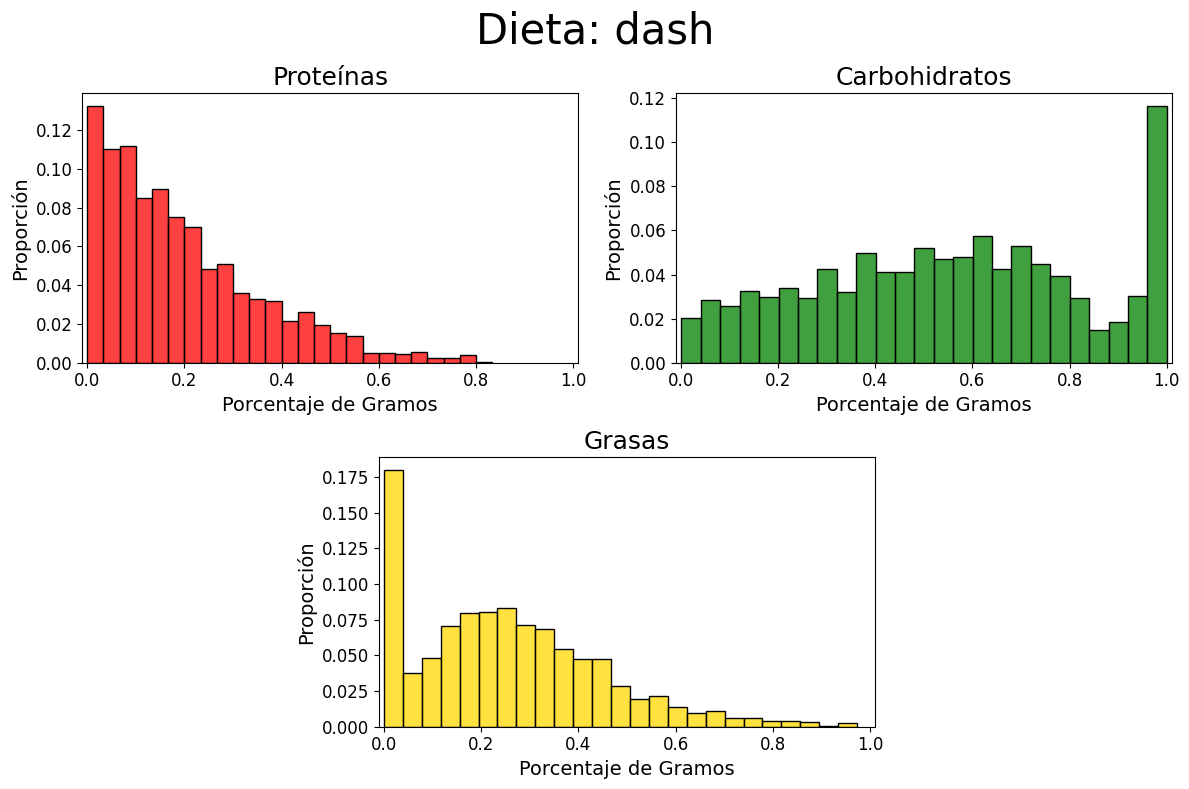
\includegraphics[width=0.75\textwidth]{Resources/2_03_plot_01.png}
        \end{center}
    \end{frame}

    \begin{frame}{Estadísticos Estratificados [Keto]}
        El $50\%$ de sus macronutrientes son grasas, esto 
        se relaciona con el hecho de que se intenta inducir 
        la ketosis; el $30\%$ son proteínas, notando que se 
        intenta reducir el consumo de carbohidratos; y el 
        $20\%$ son carbohidratos
        \begin{center}
            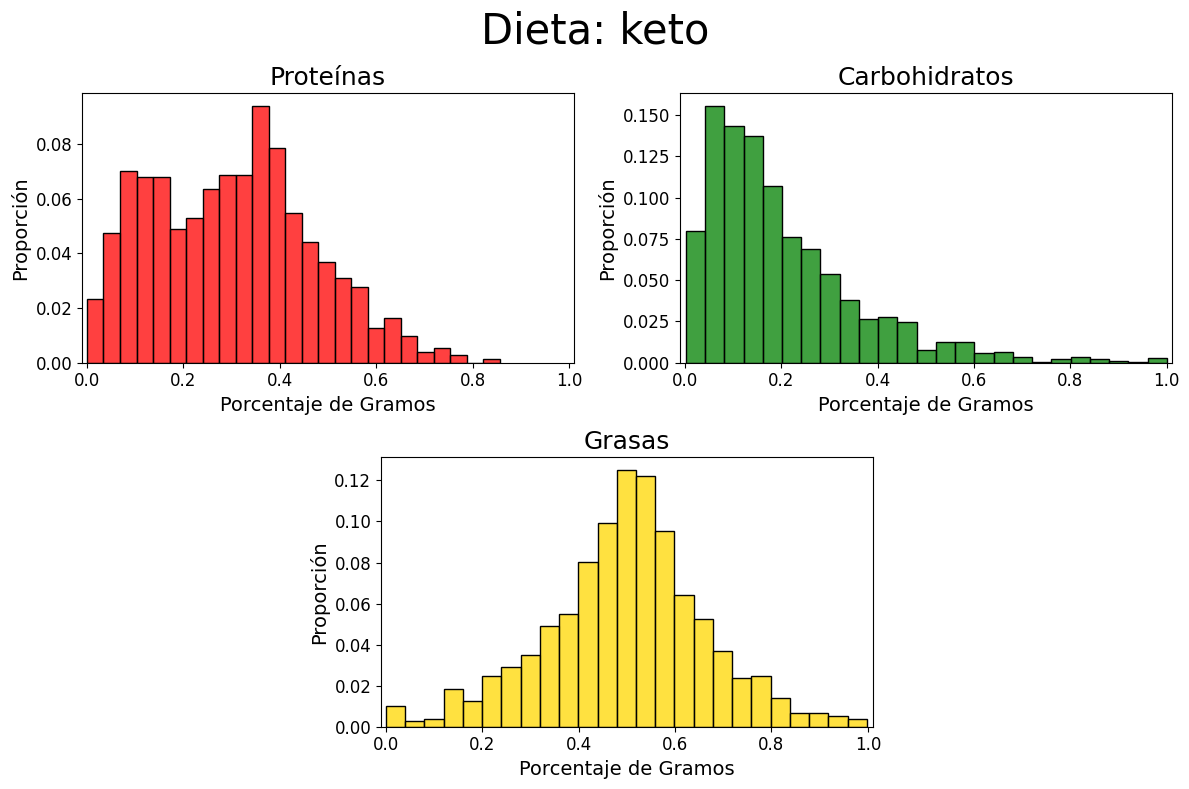
\includegraphics[width=0.75\textwidth]{Resources/2_03_plot_02.png}
        \end{center}
    \end{frame}

    \begin{frame}{Estadísticos Estratificados [Mediterránea]}
        El $42\%$ de sus macronutrientes son carbohidratos, esto 
        debido a un alto consumo de productos como frutas, vegetales 
        y granos enteros; el $30\%$ son grasas, por un alto consumo de 
        nueces y aceites; y el $28\%$ son proteínas, por un 
        consumo moderado de pescado y aves, y bajo en carnes rojas
        \begin{center}
            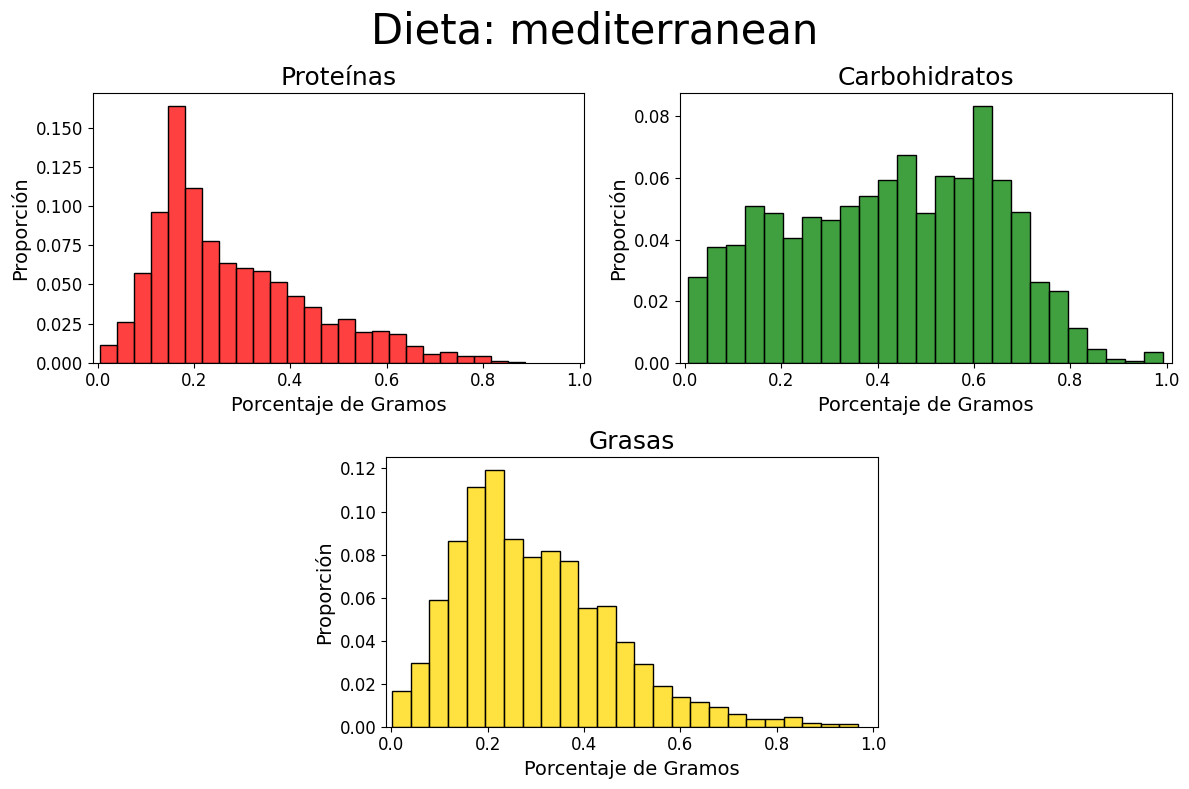
\includegraphics[width=0.75\textwidth]{Resources/2_03_plot_03.png}
        \end{center}
    \end{frame}

    \begin{frame}{Estadísticos Estratificados [Paleo]}
        El $38\%$ de sus macronutrientes son grasas y el 
        $37\%$ son carbohidratos, esto se relaciona con 
        el consumo de productos como frutas, vegetales, 
        nueces y semillas; y el $25\%$ son proteínas cuyas 
        principales fuentes son carnes margas y pescado
        \begin{center}
            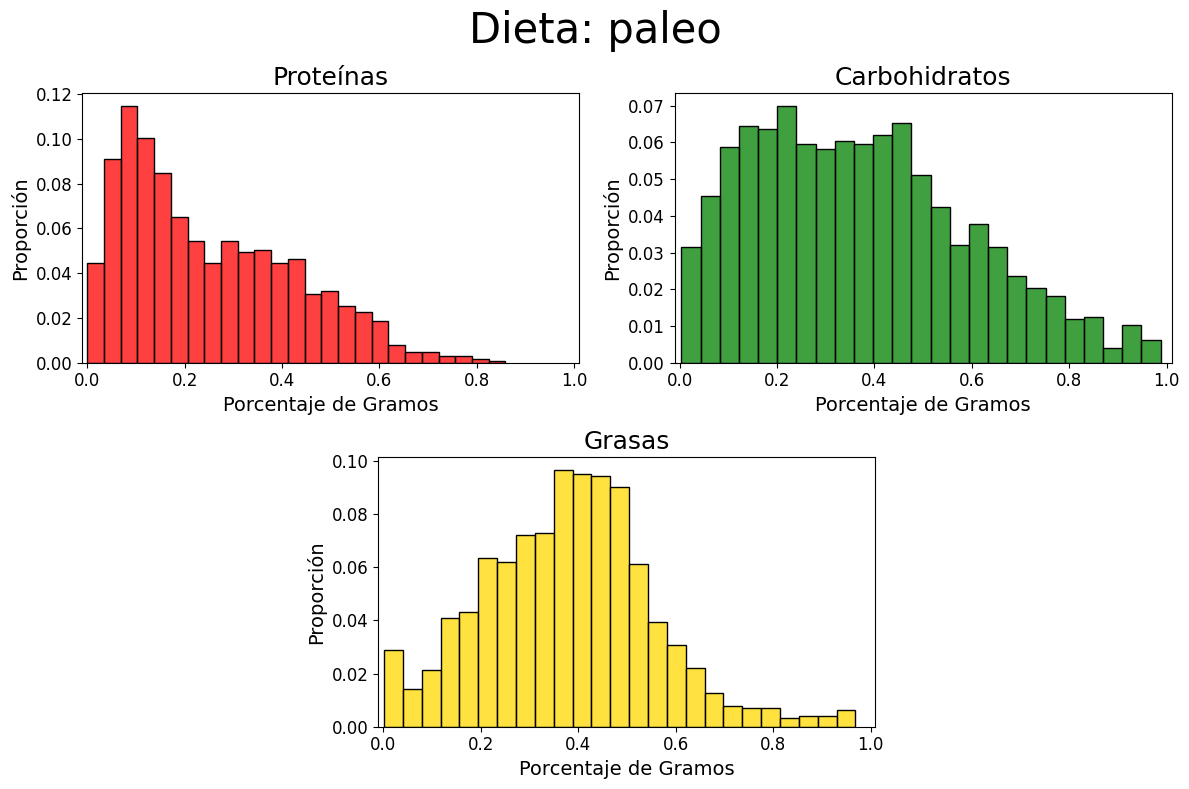
\includegraphics[width=0.75\textwidth]{Resources/2_03_plot_04.png}
        \end{center}
    \end{frame}

    \begin{frame}{Estadísticos Estratificados [Vegana]}
        El $60\%$ de sus macronutrientes son carbohidratos, 
        que provienen de fuentes vegetales; el $25\%$ son 
        grasas, relacionadas con el consumo de nueces y semillas; 
        y el $15\%$ son proteínas, esto debido a un nulo consumo 
        de alimentos de origen animal
        \begin{center}
            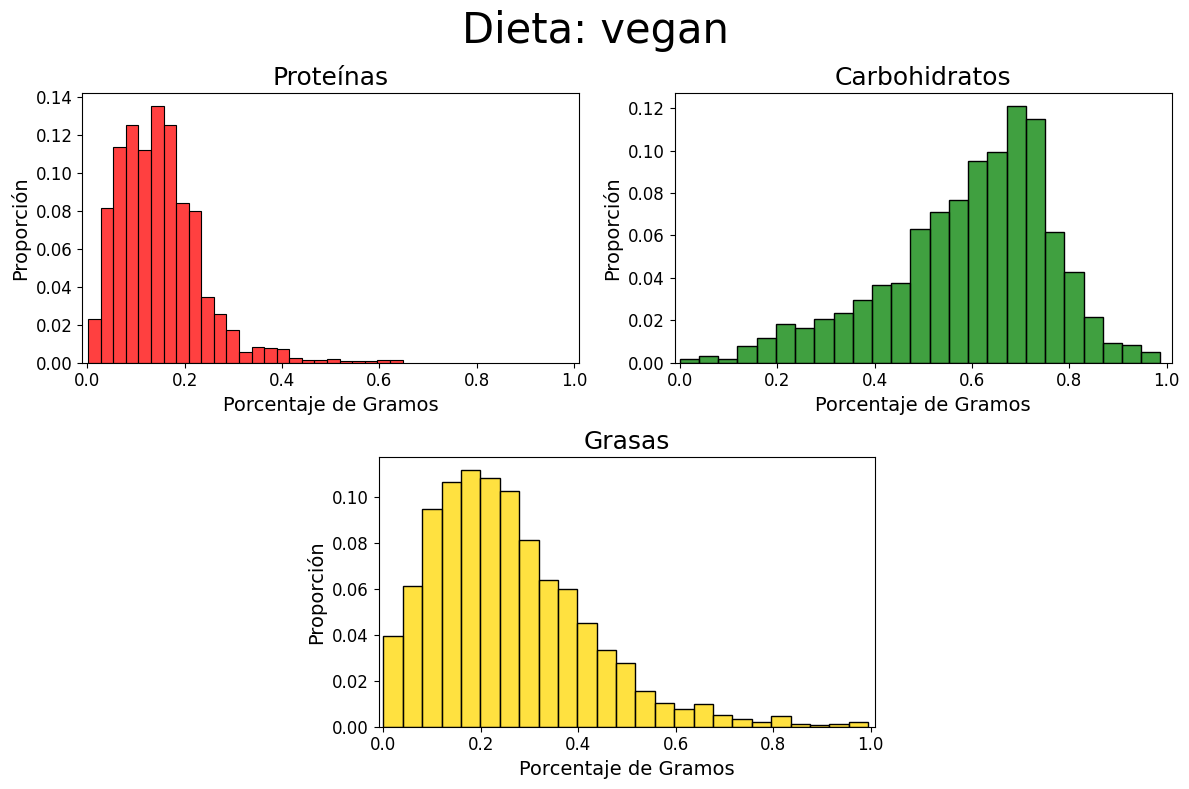
\includegraphics[width=0.75\textwidth]{Resources/2_03_plot_05.png}
        \end{center} 
    \end{frame}

    \begin{frame}{Estadísticos Estratificados [General]}
        \begin{center}
            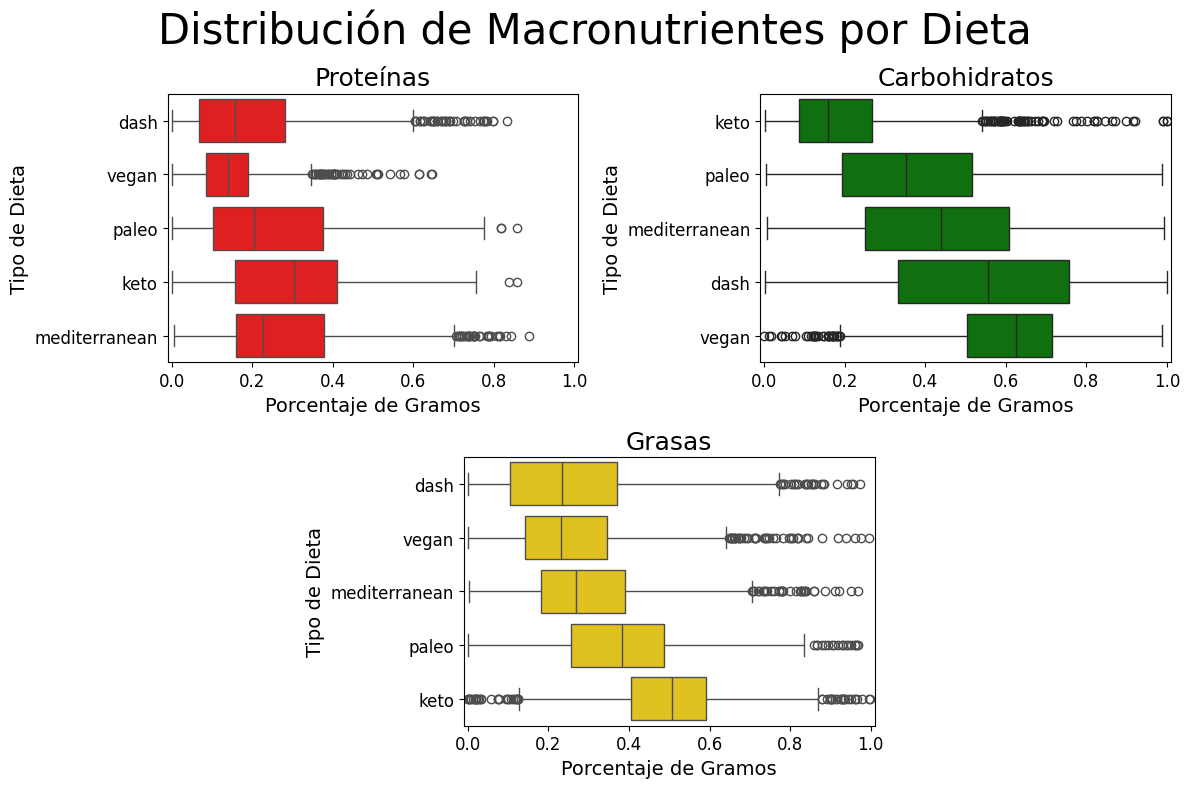
\includegraphics[width=0.9\textwidth]{Resources/2_03_plot_06.png}
        \end{center}
    \end{frame}

    \section{Muestreo e Intervalos de Confianza}

    \begin{frame}{Generalidades del Muestreo}
        \begin{itemize}
            \item Para ambos muestreos, se usó la 
            variable de \emph{Carbs(g)}. Realizándose 
            de tamaño $50$
            \item Para el muestreo estratificado, 
            se calcularon primero las proporciones 
            de las diferentes clases en \emph{Diet\_type}
        \end{itemize}
    \end{frame}

    \begin{frame}{Muestreo Aleatorio Simple [I]}
        \begin{center}
            \begin{tabular}{|c|c|c|c|c|}
                \hline
                Marca de Clase & Puntaje Z & \makecell{Frecuencia\\Absoluta} & \makecell{Frecuencia\\Relativa} & \makecell{Frecuencia\\Acumulada} \\
                \hline
                0.071112 & -1.519335 & 6  & 0.12 & 0.12 \\
                0.209217 & -0.958601 & 8  & 0.16 & 0.28 \\
                0.347321 & -0.397868 & 10 & 0.20 & 0.48 \\
                0.485426 &  0.162865 & 8  & 0.16 & 0.64 \\
                0.623530 &  0.723599 & 11 & 0.22 & 0.86 \\
                0.761635 &  1.284332 & 4  & 0.08 & 0.94 \\
                0.899740 &  1.845065 & 3  & 0.06 & 1.00 \\
                \hline
            \end{tabular}
        \end{center} 
    \end{frame}
    
    \begin{frame}{Muestreo Aleatorio Simple [II]}
        \begin{center}
            \begin{tabular}{|c|cc|}
                \hline
                Estadístico & Muestral & Poblacional \\
                \hline
                Media & 0.445313 & 0.433471 \\
                $Q_1$ & 0.247271 & 0.205251 \\
                $Q_2$ & 0.465096 & 0.432028 \\
                $Q_3$ & 0.631106 & 0.635058 \\
                Desviación Estándar & 0.246293 & 0.256032 \\
                Mínimo & 0.002060 & 0.000330 \\
                Máximo & 0.968792 & 1.000000 \\
                Asimetría de Fisher & 0.077583 & 0.189556 \\
                \hline
                \end{tabular}
        \end{center}
    \end{frame}

    \begin{frame}{Muestreo Aleatorio Estratificado [I]}
        \begin{center}
            \begin{tabular}{|c|c|c|c|c|}
                \hline
                Marca de Clase & Puntaje Z & \makecell{Frecuencia\\Absoluta} & \makecell{Frecuencia\\Relativa} & \makecell{Frecuencia\\Acumulada} \\
                \hline
                0.077393 & -1.633242 & 7  & 0.14 & 0.14 \\
                0.206757 & -1.078329 & 6  & 0.12 & 0.26 \\
                0.336121 & -0.523416 & 8  & 0.16 & 0.42 \\
                0.465485 & 0.031498  & 6  & 0.12 & 0.54 \\
                0.594849 & 0.586411  & 13 & 0.26 & 0.80 \\
                0.724213 & 1.141324  & 8  & 0.16 & 0.96 \\
                0.853577 & 1.696238  & 2  & 0.04 & 1.00 \\
                \hline
            \end{tabular}
        \end{center}
    \end{frame}

    \begin{frame}{Muestreo Aleatorio Estratificado [II]}
        \begin{center}
            \begin{tabular}{|c|cc|}
                \hline
                Estadístico & Muestral & Poblacional \\
                \hline
                Media & 0.458142  & 0.433471 \\
                $Q_1$ & 0.258305 & 0.205251 \\
                $Q_2$ & 0.501985 & 0.432028 \\
                $Q_3$ & 0.650737 & 0.635058 \\
                Desviación Estándar & 0.233125 & 0.256032 \\
                Mínimo & 0.012711 & 0.000330 \\
                Máximo & 0.918259 & 1.000000 \\
                Asimetría de Fisher & -0.226386 & 0.189556 \\
                \hline
            \end{tabular}
        \end{center}
    \end{frame}

    \begin{frame}{Intervalos de Confiaza en Muestreo Aleatorio}
        \begin{center}
            \begin{tabular}{|c|c|c|}
                \hline
                Nivel de Confianza & Límite Inferior & Límite Superior \\
                \hline
                $85\%$ & 0.395173 & 0.495454 \\
                $95\%$ & 0.377046 & 0.513581 \\
                $99\%$ & 0.355595 & 0.535032 \\
                \hline
            \end{tabular}
        \end{center}      
    \end{frame}

    \begin{frame}{Intervalos de Confiaza en Muestreo Estratificado}
        \begin{center}
            \begin{tabular}{|c|c|c|}
                \hline
                Nivel de Confianza & Límite Inferior & Límite Superior \\
                \hline
                $85\%$ & 0.410682 & 0.505602 \\
                $95\%$ & 0.393524 & 0.522760 \\
                $99\%$ & 0.373220 & 0.543064 \\
                \hline
                \end{tabular}
        \end{center}
    \end{frame}

    \begin{frame}{Hipótesis sobre las Medias}
            Si se usara la media como indicativo para determinar 
            si un muestreo es representativo, entonces: ¿Los muestreos 
            realizados son representativos? De forma equivalente, ¿Las 
            medias muestralas de la proporción de carbohidratos difieren 
            significativamente de la media poblacional?
    \end{frame}

    \section{Referencias Bibliográficas}

    \begin{frame}{Referencias}
        \printbibliography
    \end{frame}

\end{document}